\chapter{Các công trình nghiên cứu liên quan}
\label{chap:chap2}

Các nghiên cứu gần đây về việc tối ưu hóa hiệu suất tạo bằng chứng không kiến thức (ZKP), đặc biệt liên quan đến zk-SNARKs, có thể được phân loại chung thành hai hướng chính: tối ưu hóa ở phía back-end (hệ thống bằng chứng) và tối ưu hóa ở phía front-end (hệ thống ràng buộc/mạch để tạo bằng chứng) \cite{ernstberger2024zk} như minh hoạ ở hình \ref{fig:chapter2-SNARKs_realworld}.

% \begin{figure}[H]
%     \centering
%     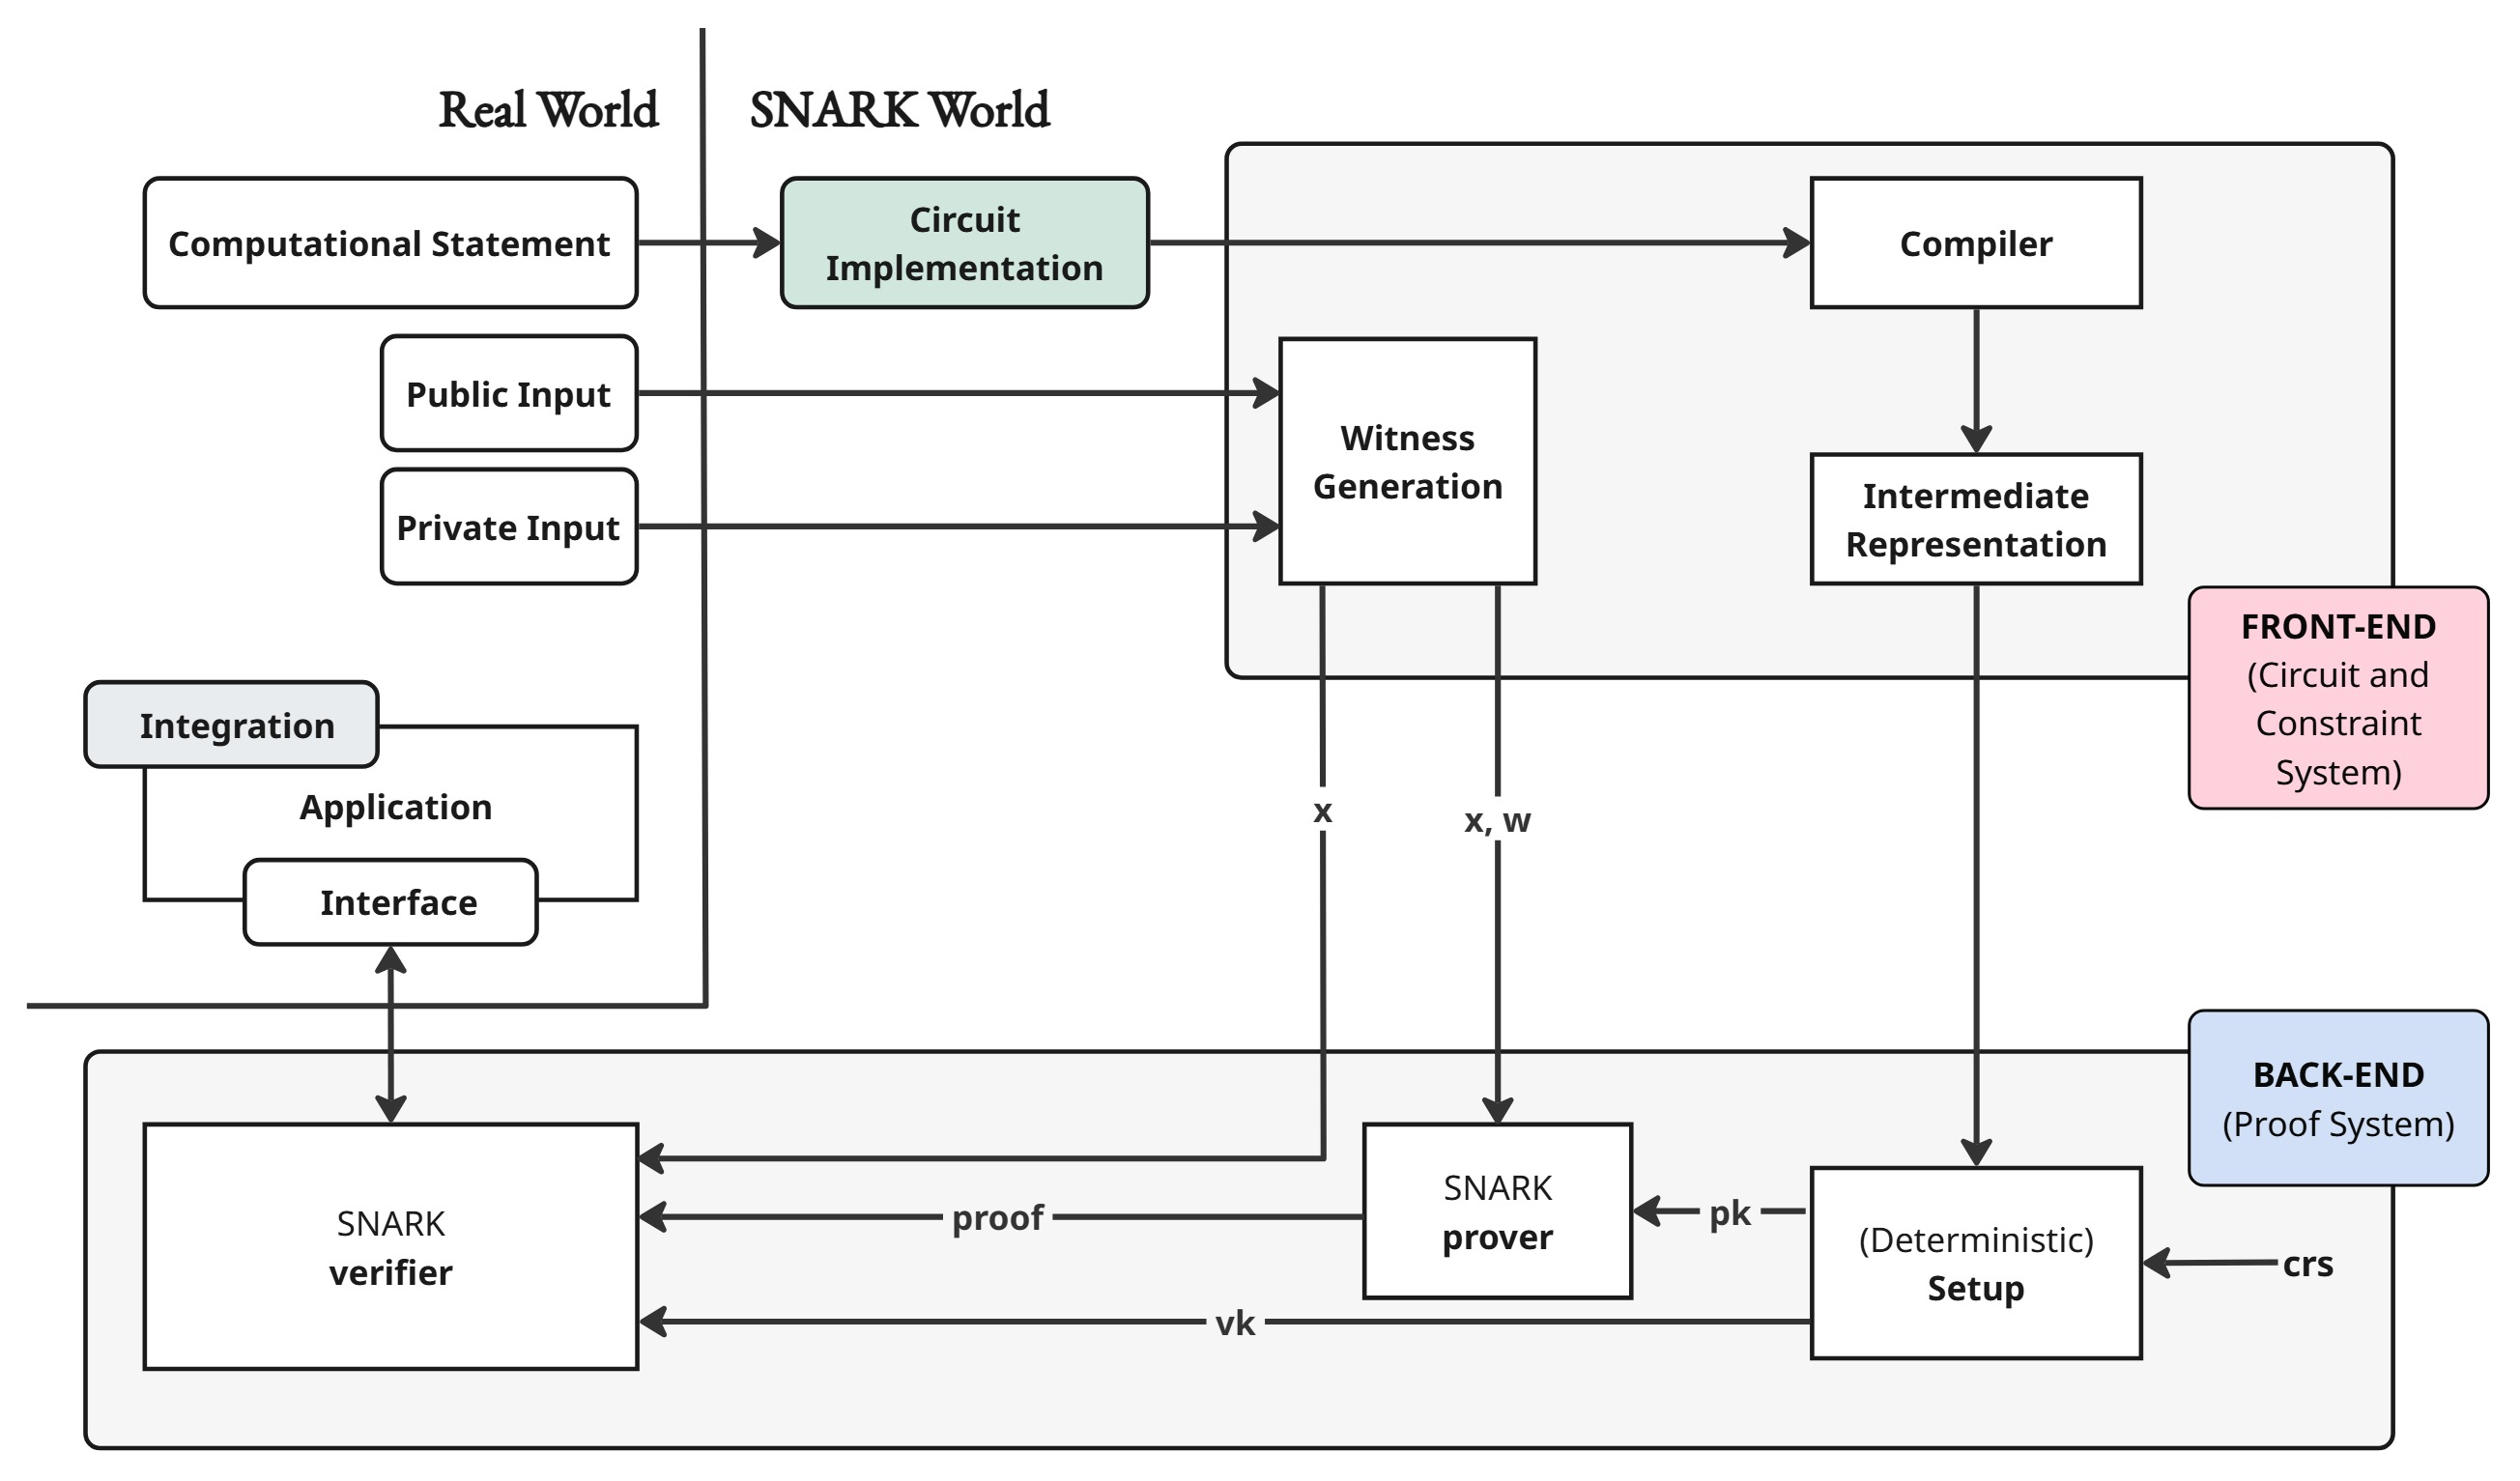
\includegraphics[width = 0.9\textwidth]{imgs/SNARKs_realworld.jpg}
%     \caption{Mối quan hệ giữa front-end, back-end của hệ thống zk-SNARKs và ứng dụng sử dụng hệ thống này}
%     \label{fig:chapter2-SNARKs_realworld}
% \end{figure}

\begin{figure}[H]
    \centering
    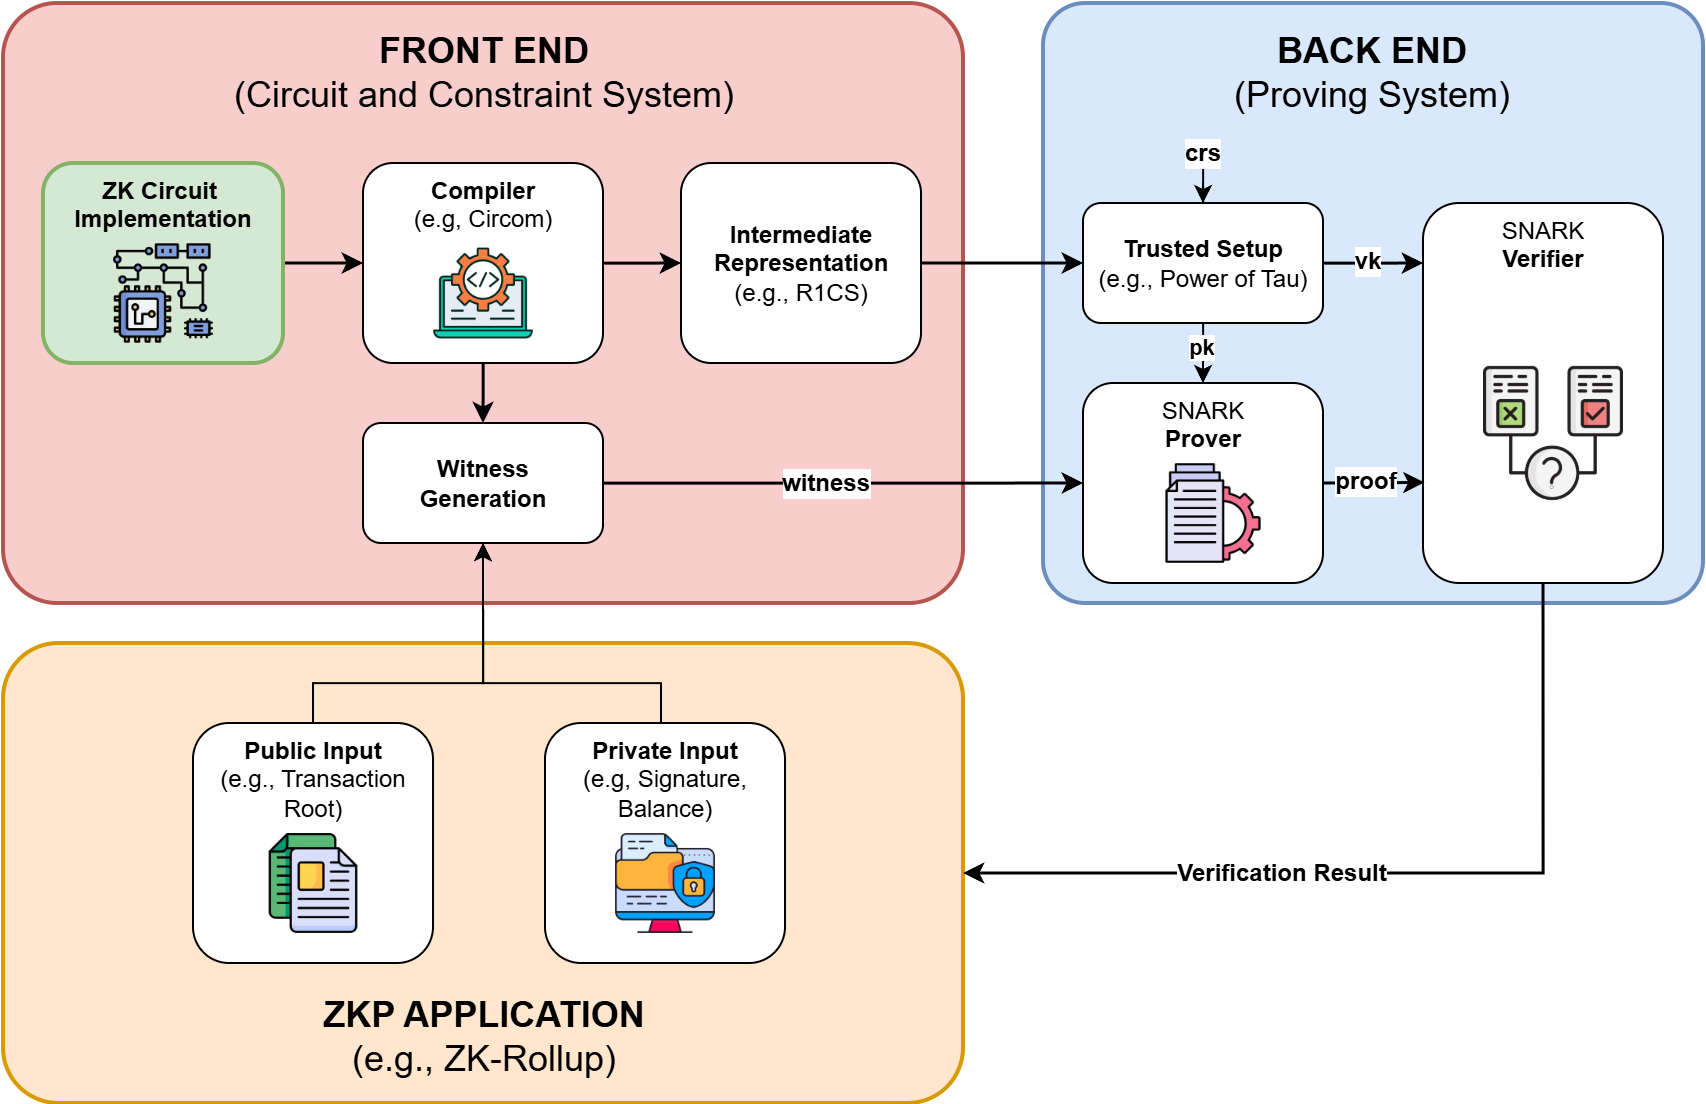
\includegraphics[width = 0.9\textwidth]{imgs/SNARKsFlow.png}
    \caption{Mối quan hệ giữa front-end, back-end của hệ thống zk-SNARKs và ứng dụng sử dụng hệ thống này}
    \label{fig:chapter2-SNARKs_realworld}
\end{figure}

\section{Tối ưu hóa back-end}
% Các nỗ lực trong lĩnh vực này tập trung vào việc đề xuất các sơ đồ ZKP mới và hiệu quả. GENES \cite{liu2025genes} là một zk-SNARK đệ quy không yêu cầu thiết lập tin cậy, giải quyết các vấn đề về thời gian tạo và xác minh bằng chứng trong các ứng dụng blockchain. Nó kết hợp nhiều phiên bản của Hệ thống Ràng buộc Bậc 1 (R1CS) thành một và sử dụng các "trợ lý" để phân phối áp lực tính toán, đạt được thời gian xác minh không đổi O(1), mặc dù kích thước bằng chứng lớn hơn so với các sơ đồ khác. HyperPlonk \cite{chen2023hyperplonk}, được phát triển dựa trên Plonk, sử dụng cấu trúc dữ liệu hypercube Boolean và cam kết đa thức đa tuyến để nâng cao hiệu suất, loại bỏ nhu cầu về các phép toán FFT phức tạp và giảm thời gian tạo bằng chứng.

% Hơn nữa, các biến thể của các sơ đồ hiện có, chẳng hạn như Groth16, đã được đề xuất để cải thiện hiệu suất. Polymath \cite{lipmaa2024polymath}, một zk-SNARK được thiết kế cho hệ thống ràng buộc Lập trình Số học Bậc 2 (SAP) thay vì R1CS của Groth16, sử dụng các sơ đồ cam kết đa thức KZG để đạt được kích thước bằng chứng ngắn hơn, đặc biệt ở các mức độ bảo mật cao hơn. Những tiến bộ này nhằm giảm thời gian tạo bằng chứng, kích thước bằng chứng và thời gian xác minh, hoặc loại bỏ nhu cầu về thiết lập tin cậy.

Những nỗ lực trong lĩnh vực này tập trung vào việc đề xuất các sơ đồ ZKP mới và hiệu quả hơn, chẳng hạn như GENES \cite{liu2025genes} -- một zk-SNARK đệ quy mới không yêu cầu thiết lập tin cậy, được thiết kế để giải quyết các vấn đề về thời gian sinh và xác minh bằng chứng trong các ứng dụng ZKP, đặc biệt là trên blockchain. GENES kết hợp các bằng chứng đệ quy, hợp nhất nhiều phiên bản của hệ thống ràng buộc bậc 1 (R1CS -- Rank 1 Constraint System) \cite{ben2013snarks} thành một, và phân bổ việc tính toán bằng cách sử dụng các ``trợ lý'' để phân tán các cam kết chứng minh. Sơ đồ ZKP này nổi bật với thời gian xác minh không đổi \(O(1)\), mặc dù có nhược điểm là kích thước bằng chứng lớn hơn so với các sơ đồ khác. 

HyperPlonk \cite{chen2023hyperplonk} là một hệ thống bằng chứng mới được phát triển dựa trên Plonk, sử dụng một cấu trúc dữ liệu đặc biệt gọi là hypercube boolean và áp dụng kỹ thuật cam kết đa thức gọi là cam kết đa thức đa tuyến để nâng cao hiệu quả. So với Plonk truyền thống, HyperPlonk mang lại một số lợi ích: loại bỏ nhu cầu tính toán FFT (Fast Fourier Transform) phức tạp và xử lý các ``cổng'' (phép toán) tùy chỉnh với độ phức tạp cao hơn một cách hiệu quả hơn. Những cải tiến này giảm đáng kể thời gian cần thiết để sinh bằng chứng. 
Bên cạnh đó, đã có nhiều nghiên cứu nhằm nâng cao các sơ đồ ZKP hiện có, chẳng hạn như Groth16, với các biến thể như Polymath \cite{lipmaa2024polymath} - một zk-SNARK được thiết kế cho hệ thống ràng buộc ``Lập Trình Số Học Bình Phương'' (SAP -- Square Arithmetic Programming) thay vì R1CS của Groth16, sử dụng các sơ đồ cam kết đa thức KZG (Kate-Zaverucha-Goldberg Polynomial Commitments). Mục tiêu chính của nó là đạt được kích thước bằng chứng ngắn hơn đáng kể, đặc biệt ở các mức độ bảo mật cao hơn. 
Mục tiêu tổng thể của những phương pháp này là giảm thời gian sinh bằng chứng, kích thước bằng chứng và thời gian xác minh, hoặc loại bỏ nhu cầu thiết lập tin cậy.

\section{Tối ưu hóa front-end}
\subsection{Tối ưu hoá về độ an toàn của mạch ZK}
% Nghiên cứu về việc tối ưu hóa các ràng buộc cho các mạch ZK đã thu hút được sự chú ý đáng kể, chủ yếu tập trung vào các khía cạnh bảo mật và tính chính xác của mạch. Điều này bao gồm việc giải quyết các mạch bị ràng buộc không đủ, chấp nhận các nhân chứng không hợp lệ, dẫn đến các lỗ hổng như khai thác trong zkSync \cite{tang2024zero}, cũng như các mạch bị ràng buộc quá mức, từ chối các nhân chứng hợp lệ, ảnh hưởng đến tính toàn vẹn của hệ thống. Các nghiên cứu đáng chú ý bao gồm AC$^4$ \cite{chen2024ac4}, một công cụ mô hình hóa các mạch Circom như các hệ thống đa thức để phát hiện các vấn đề ràng buộc, và QED$^2$ (Picus) \cite{pailoor2023automated}, kết hợp lý luận ràng buộc duy nhất nhẹ (UCP) với các bộ giải SMT để xác định các mạch bị ràng buộc không đủ. Circomspect \cite{circomspect2022}, một công cụ phân tích tĩnh, và Coda của Veridise \cite{liu2024certifying}, sử dụng xác minh chính thức, cũng đóng góp vào việc cải thiện bảo mật và tính chính xác của mạch.

% Ngoài ra, tối ưu hóa ràng buộc đã được khám phá trong các nghiên cứu như của Albert et al. \cite{albert2022distilling}, tập trung vào việc loại bỏ các ràng buộc dư thừa từ R1CS bằng cách sử dụng các hệ thống biến đổi dựa trên quy tắc và kỹ thuật loại bỏ Gaussian. Những phương pháp này nhằm giảm chi phí tính toán trong việc tạo ZKP bằng cách tối thiểu hóa các ràng buộc không cần thiết.

% Mặc dù đã có các nghiên cứu hiện có về tối ưu hóa ở phía front-end, các nghiên cứu này thường nhấn mạnh vào tính chính xác của mạch hoặc các kỹ thuật tối ưu hóa trình biên dịch tổng quát, vẫn còn một khoảng trống đáng kể trong phân tích thực nghiệm định lượng liên quan đến tác động của các tùy chọn tối ưu hóa trình biên dịch, chẳng hạn như các cờ trong Circom, đến các chỉ số hiệu suất như thời gian biên dịch và thời gian tạo bằng chứng trong các ứng dụng zk-rollup phức tạp ERC-20. Nghiên cứu của chúng tôi giải quyết khoảng trống này bằng cách định lượng các sự đánh đổi về hiệu suất và làm rõ cơ chế của tối ưu hóa --O2, nhằm giảm tổng số ràng buộc trong các phép toán mật mã cốt lõi cho các giao dịch ERC-20. Chúng tôi đề xuất một khung tối ưu hóa mạch, được hỗ trợ bởi dữ liệu thực nghiệm, để cung cấp hướng dẫn thực tiễn cho việc cải thiện hiệu suất zk-rollup thông qua quản lý ràng buộc hiệu quả. 

Nghiên cứu liên quan đến tối ưu hóa các ràng buộc cho các mạch ZK (Zero-knowledge) cũng đã thu hút nhiều sự chú ý. Tuy nhiên, hầu hết các công trình này chủ yếu tập trung vào các khía cạnh bảo mật, giải quyết các vấn đề liên quan đến tính chính xác của mạch. Điều này bao gồm việc xác định và khắc phục các vấn đề liên quan đến mạch thiếu ràng buộc (mạch chấp nhận các chứng cứ không hợp lệ, dẫn đến các lỗ hổng bảo mật nghiêm trọng, chẳng hạn như khai thác trong zkSync cho phép đánh cắp tài sản \cite{tang2024zero}) và mạch thừa ràng buộc (mạch từ chối các chứng cứ hợp lệ, ảnh hưởng đến tính hoàn chỉnh của hệ thống). Các nghiên cứu nổi bật giải quyết các vấn đề này bao gồm AC$^4$ \cite{chen2024ac4}—một công cụ mô hình hóa mạch Circom dưới dạng hệ thống đa thức và áp dụng các thuật toán đại số để kiểm tra các vấn đề thừa hoặc thiếu ràng buộc; QED$^2$ (Picus) \cite{pailoor2023automated}—một kỹ thuật và công cụ tự động được thiết kế để phát hiện các mạch ZKP thiếu ràng buộc bằng cách kết hợp lý luận ràng buộc duy nhất nhẹ (lightweight UCP -- unique constraint propagation) với các bộ giải lý thuyết module về tính thỏa được (SMT -- Satisfiability Modulo Theories); Circomspect \cite{circomspect2022}—một công cụ phân tích tĩnh (kiểm tra mã nguồn của các mạch mà không cần thực thi mã) để phân tích và xác định các lỗ hổng bảo mật trong các mạch ZKP; và Coda của Veridise \cite{liu2024certifying}—một công cụ sử dụng xác minh chính thức để kiểm tra các thuộc tính và tính chính xác của các mạch ZKP.

\subsection{Tối ưu hoá nhằm tinh gọn ràng buộc trong mạch ZK}
Ở khía cạnh tối ưu hoá hệ thống ràng buộc để gia tăng hiệu suất tạo bằng chứng ZKP, các công trình này sẽ tập trung vào việc tinh gọn, giảm thiểu số lượng ràng buộc trong các mạch ZK nhằm cải thiện khả năng tạo bằng chứng. Chẳng hạn như công trình của Albert et al. \cite{albert2022distilling}, tập trung vào việc tinh gọn các ràng buộc từ R1CS bằng cách loại bỏ các phần ràng buộc không ảnh hưởng đến bảo mật. Cụ thể, họ nhằm mục tiêu xác định và loại bỏ các ràng buộc dư thừa bằng cách sử dụng một khung cho việc giảm R1CS dựa trên hệ thống biến đổi có quy tắc và một kỹ thuật tối ưu hóa ràng buộc mới dựa trên phương pháp khử Gaussian để suy ra các ràng buộc tuyến tính từ các ràng buộc phi tuyến, với mục tiêu giảm lượng ràng buộc dư thừa trong mạch R1CS, từ đó giảm chi phí sinh bằng chứng không kiến thức. Công trình nghiên cứu này cũng đề cập rằng đây là công trình đầu tiên nghiên cứu các kỹ thuật áp dụng trên ràng buộc như một phương pháp chính thức (formal method) để giải quyết các thách thức trong việc phân tích và tối ưu hóa các giao thức ZK.

Có thể thấy rằng, mặc dù có sự tồn tại của các nghiên cứu về tối ưu hóa ở phía front-end, các nghiên cứu này thường tập trung vào tính chính xác của mạch (bảo mật). Một khoảng trống đáng kể còn tồn tại trong các nghiên cứu để tinh gọn ràng buộc tương tự như công trình của Albert et al. \cite{albert2022distilling}, nhằm mục đích gia tăng hiệu suất tạo ZKP, và cũng thiếu các cung cấp phân tích thực nghiệm định lượng về tác động của các tùy chọn tối ưu hóa biên dịch (chẳng hạn như các cờ trong Circom) lên các chỉ số hiệu suất (thời gian biên dịch và thời gian sinh bằng chứng) trong bối cảnh các ứng dụng ZK-Rollup ERC-20 phức tạp.

Nghiên cứu của khoá luận này có mục tiêu lấp đầy khoảng trống này bằng cách định lượng các đánh đổi về hiệu suất và làm rõ cơ chế tối ưu hóa --O2, tập trung vào việc giảm tổng số ràng buộc trong các phép toán mật mã cốt lõi của ZK-Rollup cho các giao dịch ERC-20. Từ đó, khoá luận đề xuất một khung tối ưu hóa mạch, hỗ trợ bởi dữ liệu thực nghiệm, để cung cấp hướng dẫn thực tiễn cho việc cải thiện hiệu suất của ZK-Rollup thông qua quản lý ràng buộc hiệu quả. Bảng \ref{tab:related_work_contributions} tóm tắt các công trình liên quan chính và xác định đóng góp của nghiên cứu trong việc tối ưu hóa các mạch ZK nhằm nâng cao hiệu suất cho ứng dụng ZKP.

\begin{table}[h]
    \centering
    \begin{tabularx}{\textwidth}{|c|>{\centering\arraybackslash}X|>{\centering\arraybackslash}X|>{\centering\arraybackslash}X|>{\centering\arraybackslash}X|>{\centering\arraybackslash}X|}
        \hline
        \textbf{Nghiên cứu} & \textbf{Cải thiện hoặc đề xuất hệ thống ZKP mới} &
        \textbf{Đảm bảo an toàn cho các mạch chứng minh không kiến thức} & \textbf{Đơn giản hoá ràng buộc cho mạch chứng minh không kiến thức} & \textbf{Phân tích đánh đổi hiệu suất khi tối ưu hoá mạch} & \textbf{Đề xuất khung tối ưu hoá mạch} \\ 
        \hline
        GENES \cite{liu2025genes} & x &  &  &  &  \\ \hline
        HyperPlonk \cite{chen2023hyperplonk} & x &  &  &  &  \\ \hline
        Polymath \cite{lipmaa2024polymath} & x &  &  &  &  \\ \hline
        AC$^4$ \cite{chen2024ac4} &  & x &  &  &  \\ \hline
        QED$^2$ (Picus) \cite{pailoor2023automated} &  & x &  &  &  \\ \hline
        Circomspect \cite{circomspect2022} &  & x &  &  &  \\ \hline
        Veridise’s Coda \cite{liu2024certifying} &  & x &  &  &  \\ \hline
        Albert et al. \cite{albert2022distilling} &  &  & x &  &  \\ \hline
        Khoá luận này &  &  & x & x & x \\
        \hline
    \end{tabularx}
    \caption{So sánh đóng góp của các công trình nghiên cứu liên quan cùng khoá luận này}
    \label{tab:related_work_contributions}
\end{table}

